% !TEX root = ../../main.tex
%

\chapter{Background} \label{chap:background}

\minitoc

Concurrency control is a crucial component in systems where multiple processes or threads simultaneously access shared resources, such as data structures, database tables, and system resources. Effective concurrency control mechanisms employ various synchronization techniques to maintain the safety and consistency of these shared resources. As noted by \citet{DBLP:books/daglib/0030596}, "Synchronization is a set of rules and mechanisms that allows the specification and implementation of sequencing properties on statements issued by the processes so that all the executions of a multiprocess program are correct."

In this chapter, we provide an overview of concurrency control mechanisms, focusing on locking. We introduce a few classical locking mechanisms, their role in synchronization and in ensuring data consistency. We discuss additional challenges brought forth by hierarchical data structures and the need for specialized locking techniques to manage concurrent access to them. Finally, we introduce the concept of multi-granularity locking and its role in balancing the trade-offs between the extremes of locking in hierarchical data structures.


\section{Hierarchical data structures}

Hierarchical data models, which have their roots in the early days of computer science, play a critical role in the representation and storage of structured information. The inception of hierarchical data can be traced back to the 1960s with the development of the Information Management System (IMS) by IBM \cite{IBMIMS}. IMS was one of the earliest database management systems designed specifically for organizing hierarchical data and was initially created to manage the complex manufacturing data associated with the Apollo space program. IMS establishes a well-defined parent-child relationship between data entities, which is a defining characteristic of hierarchical models \cite{DBLP:books/daglib/0006734}.

Over the decades, hierarchical data structures have remained pertinent, particularly in domains that require nested or tree-like relationships. They are widely utilized in XML data management, file system hierarchies, and organizational charts \cite{DBLP:books/mk/BunemanSA99}. The relevance of hierarchical models has only increased in contemporary big-data contexts, where they are often integrated with other data models, such as graphs, to address the challenges posed by the complexity and interconnectedness of modern data environments.

For instance, hierarchical data models are fundamental in NoSQL databases like Apache HBase, where the efficient storage and rapid retrieval of large-scale, semi-structured data are critical \cite{DBLP:books/daglib/0027893}. The structured nature of hierarchical models aligns well with applications in social networks, content management systems, and cloud-based storage solutions, where understanding and managing data relationships is essential.
Consequently, hierarchical data models remain foundational to modern computing, providing an effective framework for organizing and retrieving complex, nested information.

\subsection{Structure of a Hierarchy}
A hierarchy is a tree like structure with an additional property that a vertex can have multiple parents.
Formally, a hierarchy is defined as follows:

\begin{definition}
    A hierarchy is a directed graph H=(V, E, R) and R $\in$ V where
    \begin{itemize}
        \item V is a finite set of vertices.
        \item $E \subset V \times V$ is a set of directed edges where each edge (u,v) represents a parent-child relationship between vertices u (the parent) and v (the child).
        \item R is a designated root of the hierarchy such that there is a path from R to every other vertex in V.
        
    \end{itemize} 
\end{definition}



\subsection{Operations in Hierarchical Data Structures}

Hierarchical data structures support a variety of operations that enable the traversal, modification, and querying of the data. These operations are essential for managing the relationships between vertices and maintaining the integrity of the hierarchy. Some common operations on hierarchical data structures include:

\begin{itemize}

    \item \textbf{Search and Query:} Searching and querying operations involve locating specific vertices or paths within the hierarchy based on predefined criteria. These operations are essential for retrieving relevant information from the data structure. These operations result in read-only access to the hierarchy. While Data reads focus on vertices, search and query operations focus on relationships between vertices and use the edges to navigate the hierarchy.
    
    \item \textbf{Data Read and Write:} Reading and writing operations involve accessing and updating the attributes of vertices in the hierarchy. These operations are fundamental for interacting with the data and retrieving information from the structure. Often, one or more vertices are involved in a single read or write operation, depending on the specific requirements of the application. These operations do not alter the topology of the hierarchy.

    \item \textbf{Structural Modifications:} Inserting and deleting vertices or edges in a hierarchical structure can alter the topology of the hierarchy. These operations are crucial for creating new data and maintaining the integrity of the relationships between vertices. We call such operations \emph{structural modifications}.
    

\end{itemize}


\section{Need for Concurrency Control in Hierarchical Data Structures} \label{sec:multicoresystemsandconcurrencycontrol}
Locking mechanisms in hierarchical data structures are essential for ensuring data consistency and integrity in concurrent environments where multiple processes or threads may attempt to access or modify data simultaneously. Given the inherently nested and interdependent relationships among vertices in hierarchical structures, specialized locking techniques are often required to effectively manage concurrent access.

The primary objective of locking in these structures is to prevent race conditions, which occur when two or more operations interfere with one another, potentially resulting in an inconsistent or incorrect data state. By implementing appropriate locking strategies, it is possible to coordinate access to shared resources, thus safeguarding the integrity of the data and maintaining the correctness of operations performed within the hierarchy.

This work on locking focuses on a multicore system where threads concurrently access a shared graph. Such use-cases provide the possibility to use a single centralized scheduler which decides on the ordering of the lock requests. In distributed deployments like HPC clusters where the communication can be guaranteed to be quasi-instantaneous, locking can still be useful since synchronization primitives can be implemented without worrying about catastrophic network partitions. Geo-distributed graphs and synchronization are out of the scope of this work. As such, locking in any form is not an efficient solution for use-cases where the graph is geo-distributed and the communication latency (ergo the synchronization delay) is high. 

The requirement for any locking technique over graphs is to protect the vertices and edges of the graph against concurrent write access. Writes can modify the data on the vertices or add/remove edges from the graph. 

A lock protocol typically involves five main steps:

\begin{enumerate}
    \item \textbf{Requesting a Lock:} A thread initiates the locking process by submitting a request to acquire a lock on a specific set of vertices that it intends to access for a write operation. This request is an attempt to ensure that only the requesting thread can modify said vertices during the operation, thereby maintaining data integrity and avoiding interference from other concurrent operations.

    \item \textbf{Detecting Conflicts:} Upon receiving a lock request, the locking protocol detects conflicts with locks held by other threads. This step is critical to preserve mutual exclusion. If a conflict is detected, the protocol determines whether the requesting thread should proceed or be temporarily blocked.


    \item \textbf{Acquiring a Lock:}  If conflict detection confirms no overlapping locks, the locking protocol grants the requested lock, allowing the thread to proceed with its intended write operation. In cases where a conflict exists, the requesting thread is put into a blocked state, where it waits until the conflict is resolved, typically by the release of the conflicting lock. This blocking mechanism is designed to prevent busy-waiting and reduce system resource usage.

    \item \textbf{Performing an Operation:} With the lock granted, the thread performs its designated read or write operation on the locked vertices. The lock ensures that no other thread can access these vertices concurrently for a write operation. Upon completing the operation, the thread prepares to release the lock, signaling the end of its exclusive access.
    
    \item \textbf{Releasing the Lock:} After finishing the operation, the thread releases the lock on the vertices, allowing other threads to request and potentially acquire locks on the same vertices. This release phase reopens access to the locked vertices, ensuring that other threads waiting to modify or read the same graph segments can proceed according to the locking protocol's scheduling and prioritization rules.
\end{enumerate}

An implementation of a locking protocol makes a few assumptions on the implementation and use.

\begin{enumerate}
    \item \textbf{Atomicity of Lock Operations:} It is assumed that lock acquisition and release operations are atomic, meaning they are indivisible and cannot be interrupted mid-operation. This atomicity ensures that no two threads can simultaneously request and acquire a lock on the same resource, which is essential to prevent race conditions.
    
    \item \textbf{Non-Malicious Threads:} The algorithm assumes that threads behave cooperatively, following established protocols without attempting to bypass or tamper with the locking mechanism. Also, threads do not attempt to access vertices without acquiring an appropriate lock. This assumption excludes scenarios where threads might act maliciously or fail to adhere to the locking protocol, simplifying the conflict detection and lock management processes.
    
    \item  \textbf{Fairness in Lock Scheduling:} Many locking algorithms assume a fair scheduling mechanism, meaning that each lock request is eventually granted in a finite amount of time, avoiding starvation where certain threads are indefinitely blocked. This fairness ensures that all threads have equitable access to shared resources, which is particularly important in high-throughput environments like HPC.

    \item \textbf{Deterministic Conflict Detection:}  It is assumed that the conflict detection mechanism can deterministically identify conflicts between lock requests and consistently enforce access restrictions. This assumption is crucial for ensuring that threads either proceed with their operations or are correctly blocked when a conflict is detected.
    
    \item \textbf{Consistency of Shared State:} The algorithm assumes that the state of shared data remains consistent and is correctly updated before each lock release. This assumption ensures that subsequent operations access an accurate version of the graph data, preventing issues such as stale data reads or lost updates.
\end{enumerate}


Together, these prerequisite steps and assumptions form the foundation for effective concurrency management, allowing the locking algorithm to maintain data integrity while maximizing system efficiency.


% An application that uses CALock can have multiple threads that concurrently access the graph. Each thread can request a lock on a set of vertices(lock targets). The locking algorithm then grants the lock request by locking a single vertex(the guard), that protects the set of vertices.
% Once a thread identifies a guard and issues a lock request, the guard cannot to be changed i.e. the guard is fixed for the duration of the lock. This is to ensure that the lock grain remains consistent for the duration of the lock. If a conflict is detected between two lock requests, one of the threads is blocked until it is notified to resume i.e. no busy waiting. In our design, we assume that the threads are not malicious and do not try to circumvent the locking and conflict detection mechanism



\section{Role of Locking in Concurrency Control}
As computing systems increasingly rely on concurrent processing, effective concurrency control mechanisms are essential for ensuring the integrity and reliability of shared resources. Locking mechanisms are a foundational strategy in managing access to these resources, allowing for mutual exclusion and preventing conflicts that can arise when multiple threads attempt to modify shared data simultaneously.

In this section, we explore the critical roles that locking plays in concurrency control. We first examine how locks prevent race conditions by ensuring that only one thread can modify shared data at a time. Next, we discuss the importance of locks in maintaining data consistency through atomic operations. Finally, we address the challenges of deadlock prevention and the strategies that can be employed to minimize this risk. Through this overview, we highlight the significance of locking mechanisms in supporting robust and reliable concurrent programming.


\subsection{Safety}

Race conditions are a fundamental concern in concurrent programming, occurring when multiple threads access and modify shared data simultaneously without proper synchronization mechanisms in place. This lack of coordination can lead to unpredictable and erroneous outcomes, as the final state of the data may depend on the timing of the thread executions rather than a well-defined sequence of operations. Locks play a critical role in preventing race conditions by ensuring that only one thread can modify shared data at any given time. By acquiring a lock before accessing the data, a thread effectively prevents other threads from making concurrent modifications, thereby establishing a controlled environment for data access.

The implementation of locks creates critical sections—regions of code that must be executed by only one thread at a time. When a thread acquires a lock, it enters the critical section and can safely perform operations on the shared data, knowing that no other thread can interfere during this period. Once the operations are complete, the thread releases the lock, allowing other waiting threads to enter the critical section. This mechanism not only prevents race conditions but also enhances the reliability of concurrent programs, as it provides a straightforward method for enforcing mutually exclusive access to shared resources.

% \subsection{Ensuring Data Consistency}

Locks are instrumental in ensuring data consistency across concurrent operations. In computing, consistency refers to the property that shared data remains in a valid state throughout the execution of concurrent transactions. Locks help maintain this consistency by enforcing atomicity, a key aspect of transaction management that dictates that operations on shared data should be treated as indivisible units. This means that a series of operations can either be completed in their entirety or not executed at all, effectively preventing intermediate states that could lead to data corruption.

For instance, consider a banking application where a user initiates a transfer of funds from one account to another. This operation typically involves several steps: debiting the source account, crediting the destination account, and possibly updating transaction logs. If these operations are interrupted by another thread accessing the same accounts, the integrity of the transaction may be compromised, leading to scenarios such as double spending or incorrect balances. By using locks to protect these operations, the system ensures that each transfer is executed atomically, thus maintaining the integrity and consistency of the financial data. This mechanism is crucial not only for ensuring correctness in transactional systems but also for building trust in applications that rely on shared data.


\subsection{Liveness}

While locks are essential for ensuring safe and consistent access to shared resources, their improper use can lead to deadlocks—situations where two or more threads are waiting indefinitely for each other to release locks, thereby causing a standstill in program execution. Deadlocks can severely impact system performance and responsiveness, making it critical to implement strategies for their prevention.

Several techniques can be employed to mitigate the risk of deadlocks in systems utilizing locks. One common approach is lock ordering, which mandates that all threads acquire locks in a predefined sequence. By adhering to a global order for lock acquisition, the system effectively eliminates circular wait conditions, which are a primary cause of deadlocks. For example, if Thread A acquires Lock 1 and Thread B acquires Lock 2, both threads should be programmed to request subsequent locks in the same order. This strategy significantly reduces the chances of deadlock occurrences, as it prevents the formation of cycles in the waiting graph.

Another useful technique is the implementation of timeout mechanisms. By allowing threads to specify a maximum waiting period for acquiring locks, the system can reduce the likelihood of indefinite waiting. If a thread cannot acquire the desired lock within the specified time-frame, it can abandon its attempt and either retry later or perform alternative actions. This not only aids in breaking potential deadlocks but also enhances overall system responsiveness, as it prevents threads from being indefinitely stalled.



\section{Requirements} \label{sec:requirements}

The design of a locking mechanism for hierarchical data structures must satisfy several key requirements to ensure the correctness, efficiency, and scalability of the system. These requirements are essential for guiding the development and evaluation of the locking algorithm. 
They can be categorized into four main areas of concern:

\begin{itemize}
    \item[\Ra] \emph{Identifying a lock guard for every vertex of a hierarchy}. For a given lock target, the lock protocol must effectively and efficiently identify the appropriate lock guard that protects this target. This is essential to ensure that the lock granularity can be minimized while maintaining data consistency. If a protocol fails to identify an appropriate guard, it may lead to unnecessary contention and reduced concurrency.

    \item[\Rb] \emph{Finding an appropriate lock guard for a request}. When a thread requests a lock on a set of lock targets, the locking protocol must determine an appropriate lock guard for this request that maximizes concurrency and minimizes contention with other lock requests. This involves considering the topology of the hierarchy and the relationships between vertices to minimize conflicts where two threads request locks on overlapping grains.
    
    \item[\Rc] \emph{Efficiently detecting conflicts between locks.} Since a correct locking protocol is workload agnostic, it must allow a thread to efficiently detect conflicts with other lock requests. In MGL, this involves testing the ancestor-descendant relationships between two lock guards which in turn implies grain overlap. If a thread requests a lock on a vertex, then to prevent conflicts, a locking protocol must ensure that no ancestor or descendant of this vertex is locked by another thread in a conflicting mode. 
    
    \item[\Rd] \emph{Housekeeping the metadata required to implement the locking protocol.} The additional metadata required to implement the locking protocol and the conflict detection mechanism must be managed efficiently to minimize the overhead of using that particular locking protocol. If the metadata management is prohibitively expensive for certain workloads, the locking protocol may not be practical for real-world applications that encounter those workloads. 
\end{itemize}


% \section{Concurrency control though general locking}
% The form of synchronization studied in our work is \emph{competition synchronization} where multiple threads compete for access to shared resources. 
% Locking is one of the primary mechanisms used to ensure data integrity and consistency in such environments.
% It restricts access to a shared data structure by multiple threads or processes to prevent conflicts and ensures that no more than one writer can modify the data at a time. 
% Here’s a high-level overview of how locking works and its role in concurrency control:

% \subsection{Mutex (Mutual Exclusion) Locks}

% One of the most fundamental forms of locking is the mutex lock, short for \emph{mutual exclusion} lock. A mutex lock is designed to provide exclusive access to a shared resource by ensuring that at most one thread can acquire the lock at any given time. When a thread requests a mutex lock, it must wait if another thread currently holds the lock. Once the holding thread releases the lock, the waiting thread can then acquire it, thereby gaining access to the shared resource.

% Mutex locks are widely used in various concurrent programming scenarios, as they effectively prevent race conditions—situations where the outcome of operations depends on the unpredictable timing of thread execution. By enforcing mutual exclusion, mutex locks ensure that critical sections of code, where shared resources are accessed or modified, are executed by only one thread at a time.

% \begin{lstlisting}
%     std::mutex mtx;
%     int counter = 0;

%     void increment(int iterations) {
%         for (int i = 0; i < iterations; ++i) {
%             std::lock_guard<std::mutex> lock(mtx);
%             ++counter;
%         }
%     }
% \end{lstlisting}

% While mutex locks are effective for synchronization, they also introduce potential drawbacks, such as lock contention and the risk of deadlocks. Lock contention occurs when multiple threads attempt to acquire the same mutex lock simultaneously, resulting in delays and reduced performance. Deadlocks can arise when two or more threads are waiting indefinitely for locks held by each other, creating a cycle of dependency.

% Mutex locks provide a straightforward mechanism for managing access to shared resources, although careful design is required to mitigate their inherent limitations.



% \subsection{Reader-Writer Locks}
% Another important synchronization mechanism is the reader-writer lock also called shared-exclusive lock. Reader-writer locks are designed to allow concurrent access to shared resources while differentiating between two types of operations: read and write. This differentiation facilitates improved performance in scenarios where read operations significantly outnumber write operations.

% A reader-writer lock enables multiple threads to simultaneously acquire the lock for reading, provided that no thread is currently writing. This means that as long as the resource is not being modified, multiple readers can access the resource concurrently, enhancing throughput. Conversely, when a thread intends to write to the shared resource, it must acquire exclusive access, which means that no other readers or writers can access the resource during this time. This mechanism prevents data inconsistency that could arise from simultaneous read and write operations.

% \begin{lstlisting}
%     ReaderWriterLock rwlock;
%     int counter = 0;

%     void reader(int iterations) {
%         for (int i = 0; i < iterations; ++i) {
%             rwlock.reader_lock();
%             // Read operation (e.g., print counter)
%             std::cout << "Read counter: " << counter << std::endl;
%             rwlock.reader_unlock();
%         }
%     }

%     void writer(int iterations) {
%         for (int i = 0; i < iterations; ++i) {
%             rwlock.writer_lock();
%             ++counter;
%             rwlock.writer_unlock();
%         }
%     }
% \end{lstlisting}

% The structure of reader-writer locks generally consists of two types of locks: a read lock and a write lock. When a thread requests a read lock, it can proceed if no write lock is held; however, if a write lock is active, the requesting thread must wait. When a thread requests a write lock, it must wait until there are no active readers or writers.

% While reader-writer locks can enhance performance by allowing multiple concurrent reads, they introduce complexity in terms of synchronization. One potential challenge is ensuring fairness, as a prolonged sequence of read operations could lead to writer starvation, where a waiting writer is indefinitely delayed because readers continue to acquire the read lock. Additionally, if not managed carefully, reader-writer locks can still suffer from lock contention and deadlocks.

% Reader-writer locks are powerful for optimizing access to shared resources, particularly in read-heavy environments. They allow for greater concurrency compared to mutex locks, but their implementation requires careful consideration to avoid potential pitfalls.



% Spinlocks:
% \begin{lstlisting}
%     Spinlock spinlock;
%     int counter = 0;

%     void increment(int iterations) {
%         for (int i = 0; i < iterations; ++i) {
%             spinlock.lock();
%             ++counter;
%             spinlock.unlock();
%         }
%     }
% \end{lstlisting}
% Spinlocks are a type of lock where a thread repeatedly checks if the lock is available, consuming CPU cycles.
% They are useful in scenarios where the wait time is expected to be very short.
% Example in C++:

% Improving Performance:

% While locks can introduce overhead, they are essential for ensuring the correctness of concurrent programs.
% Using appropriate locking mechanisms (e.g., read-write locks) can help balance performance and data integrity.
% Example Scenario
% Consider a shared data structure like a linked list that multiple threads need to update:

% % In this example, the std::lock_guard ensures that the mutex is automatically released when the function exits, even if an exception is thrown.

% Conclusion
% Locking is a fundamental technique in concurrency control that helps ensure the integrity and consistency of shared data structures in multi-threaded environments. By understanding and correctly implementing locking mechanisms, you can prevent race conditions, maintain data consistency, and improve the overall reliability of your concurrent programs.

\section{Locking in Hierarchical Data Structures}
Before delving into the detailed discussion of locking and its relevance to hierarchical data, it is essential to establish the foundational terminology that will be used throughout this thesis. Hierarchical locking, as a mechanism for managing concurrent access to data structured in a hierarchy, involves a variety of concepts that require precise definitions to avoid ambiguity and ensure clarity.

In particular, concepts like "lock grain," which describe levels of granularity in hierarchical locking, are critical for understanding the nuances of how concurrency is managed in hierarchical and graph-based data models. While some of these terms are standard in the literature, others are specific to the context of this thesis, reflecting the unique challenges and solutions presented by hierarchical data structures.

\subsection{Key terms in hierarchical locking}

Understanding the terminology associated with hierarchical locking is crucial for effectively discussing and implementing locking mechanisms in hierarchical data structures. Below are some fundamental terms used in this context:

\subsubsection{Lock Target} The lock target refers to a specific vertex or a set of vertices within the hierarchy that a lock is intended to protect. Identifying the appropriate lock target is critical for preventing conflicts and ensuring that concurrent operations do not interfere with each other. The selection of lock targets can influence the efficiency of locking protocols, as improper targeting may lead to unnecessary contention or reduced concurrency.

\subsubsection{Lock Guard} The lock guard is an entity that serves as the point of synchronization for a given set of lock targets. When a thread wishes to access a particular target, it must acquire the corresponding lock guard to ensure exclusive access to the target. The lock guard acts as a sentinel, preventing other threads from modifying the protected data until the lock is released. The mapping between a lock target and its corresponding lock guard is dependent on the locking protocol. We shall see examples of this in Chapter \ref{chap:relatedwork}.

\subsubsection{Lock Grain and Granularity} Lock grain refers to the scope of the data that is being locked when a lock is acquired on a guard. The size of the grain is called its \emph{granularity}. In hierarchical locking, this can vary from coarse-grained locks that encompass large portions of the hierarchy (e.g. entire subgraphs) per lock guard to fine-grained locks that target individual vertices or smaller groups of vertices per lock guard. The choice of lock grain (resp. granularity) directly impacts the level of concurrency and performance in a system; while fine-grained locks allow for greater parallelism, they can introduce additional complexity in managing locks.


\subsection{Classical locking approaches for connected data}
A common approach for synchronization in connected data, like graphs, is lock coupling \cite{DBLP:journals/acta/BayerS77}, also known as hand-over-hand locking. In hand-over-hand locking, a thread locks a vertex before traversing to one of its children in the structure, unlocking the parent once the child is locked. 
This allows for per vertex synchronization, which improves concurrency by permitting multiple threads to work on different parts of the hierarchy simultaneously. 
However, as \citet{LeisH019} show, lock coupling can lead to suboptimal locking performance on modern hardware. 


An alternative to lock coupling, targeted specially for B-trees is a variant called B-Link tree \cite{LehmanY81}. A B-link tree is an extension of the B-tree data structure that adds sibling pointers to improve concurrency and simplify lock management in multithreaded environments. In a traditional B-tree, nodes are connected in a hierarchical structure with each node containing keys and pointers to child nodes, but concurrent modifications require complex locking strategies to maintain consistency. B-link trees address this by adding \emph{right sibling} pointers between nodes at the same level, allowing threads to traverse the tree even during insertions or deletions without needing to lock the entire structure. This enables more efficient concurrent access, as threads encountering locked nodes can follow sibling links to find the next valid node. B-link trees require additional mechanisms to ensure that pointer updates are atomic since multiple threads may attempt to modify the same pointers concurrently. Additionally, this approach is only applicable to tree-based structures and is not be directly transferable to other hierarchical data models.


Classical locking techniques for hierarchical data structures are often designed with a synchronization hypothesis. A hypothesis defines how and when synchronization mechanisms (like locks, barriers, or other coordination tools) are applied to ensure threads or processes do not interfere with each other. Lock coupling uses a simple hypothesis that a thread must acquire a lock on a vertex before traversing to its children. B-link trees introduce a more sophisticated hypothesis by allowing threads to follow sibling pointers when encountering locked nodes, thus reducing contention and improving concurrency. Such design choices limit their use in general purpose applications where the topology of a linked structure is not known a priori. 

\subsection{Fixed Grain locking}
Unlike classical approaches which define a specific synchronization mechanism, reader-writer locks are often appropriated for hierarchical data by associating a lock guard for a predefined set of lock targets. For example, a unique lock guard can be assigned for all vertices of the same depth from the root of the hierarchy. Since this guard is fixed and does not depend on the lock request, we refer to this as \emph{fixed-grain locking}.

Fixed-grain locking has two extremes: We can either have a single lock guard for all the vertices in the hierarchy (coarse-grain locking) or a unique lock guard for each target vertex (fine-grain locking).
% The granularity of a lock determines the degree of concurrency and the amount of contention in the system. 



\begin{figure}[H]
    \captionsetup{justification=centering}
    \centering
    \begin{subfigure}{.49\textwidth}
        \centering
        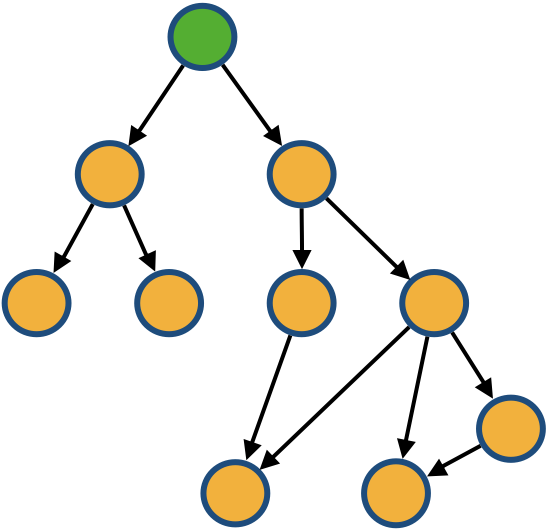
\includegraphics[width=.7\columnwidth]{figures/CoarseGrainedLockingTree}
        \caption{Coarse-grain lock}        
        \label{fig:fixedLockGrainsCoarse}
    \end{subfigure}
    \begin{subfigure}{.49\textwidth}
        \centering
        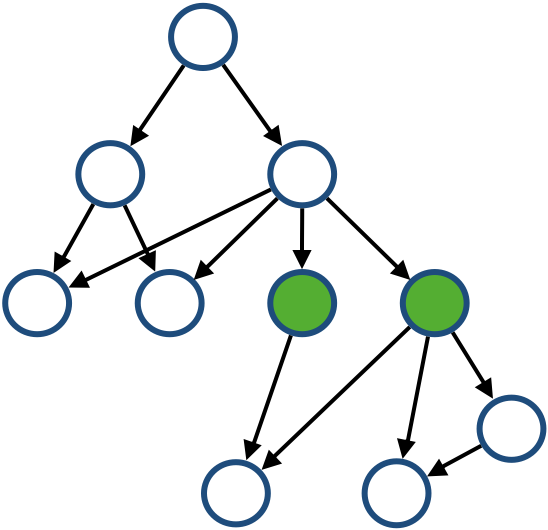
\includegraphics[width=.7\columnwidth]{figures/FineGrainLockingTree}
        \caption{Fine-grain locks}
        \label{fig:fixedLockGrainsFine}
    \end{subfigure}
    
    \label{fig:fixedLockGrains}
\caption{Fixed-grain locks in a hierarchical data structure (lock guard in green and the corresponding grain in yellow).}
\end{figure}


\paragraph{Coarse-Grain Locking}
An oversimplified approach for correct thread synchronization is to guard an entire hierarchy with a reader-writer lock such that any thread accessing the hierarchy must first acquire this lock.
This approach is called \emph{coarse-grain locking} and is shown in Figure \ref{fig:fixedLockGrainsCoarse}.
A thread that wishes to access any vertex in the hierarchy must first acquire a lock on the entire data structure and consequently block all other writers until it releases this lock. 
Coarse-grain locking is simple to implement and has extremely low locking overhead but suffers from the highest possible contention as all threads must acquire the same lock to access any part of the hierarchy. 


\paragraph{Fine-Grain Locking}
Another well known approach to locking is when every target vertex is its own guard i.e. every vertex has its own unique lock. 
We call this \emph{fine-grain locking}.
As shown in Figure \ref{fig:fixedLockGrainsFine}, vertices are locked individually and a thread that needs to access multiple vertices must acquire multiple locks. 
Fine-grain locking has the advantage of reducing contention as threads can access disjoint parts of the hierarchy concurrently. 
However, the overhead of acquiring multiple locks makes this approach less efficient. 


The approaches shown in Figures \ref{fig:fixedLockGrainsCoarse} and \ref{fig:fixedLockGrainsFine} have their own trade-offs. 
Coarse-grain locking causes contention by unnecessarily blocking threads that access disjoint parts of the hierarchy. 
Fine-grain locking, on the other hand, introduces significant overhead due to the need to acquire multiple locks for accessing multiple vertices with the additional requirement of deadlock detection and prevention/resolution.

\subsection{Multi-Granularity Locking}
In contrast to fixed-grain locking, multi-granularity locking adapts the granularity of locks based on the structure of the hierarchy and the lock request. 
According to \citet{gray1975granularity}, "Multi-granularity locking involves locking a guard in a hierarchy such that a single lock guard is sufficient to protect all the target vertices protected by that guard i.e. a thread that requests a write (exclusive) lock on a guard vertex implicitly exclusively locks all its targets when its request is granted". 

% A vertex which a thread intends to access is called the \emph{lock target} of the thread. 
% MGL methods generally associate a lock with each vertex in the hierarchy which we call the \emph{guard} of the vertex. 
% As such, when a thread wishes to access a target, it must acquire an appropriate lock on the guard of the the target vertex. 


\emph{Multi-granularity locking} (MGL) \cite{gray1975granularity} techniques find a balance between the two extremes of fixed-grain locking based on the topology of the hierarchy.
% \emph{Multi-granularity locking} (MGL) \cite{gray1975granularity} techniques exploit the topology of the graph to identify a pertinent guard for a given target and aim to strike a balance between these two extremes. 
Since \emph{granularity} depends on the topology of the graph and on the lock request, lock requests with the same set of lock targets for different hierarchies can have different granularities, hence the name. A classical example of MGL is \emph{Intention locks} \cite{StonebrakerGranularity} which are often used in database indices to optimize hierarchical access \cite{sqlintentionlocks}. 

\begin{figure}[h]
    \captionsetup{justification=centering}
    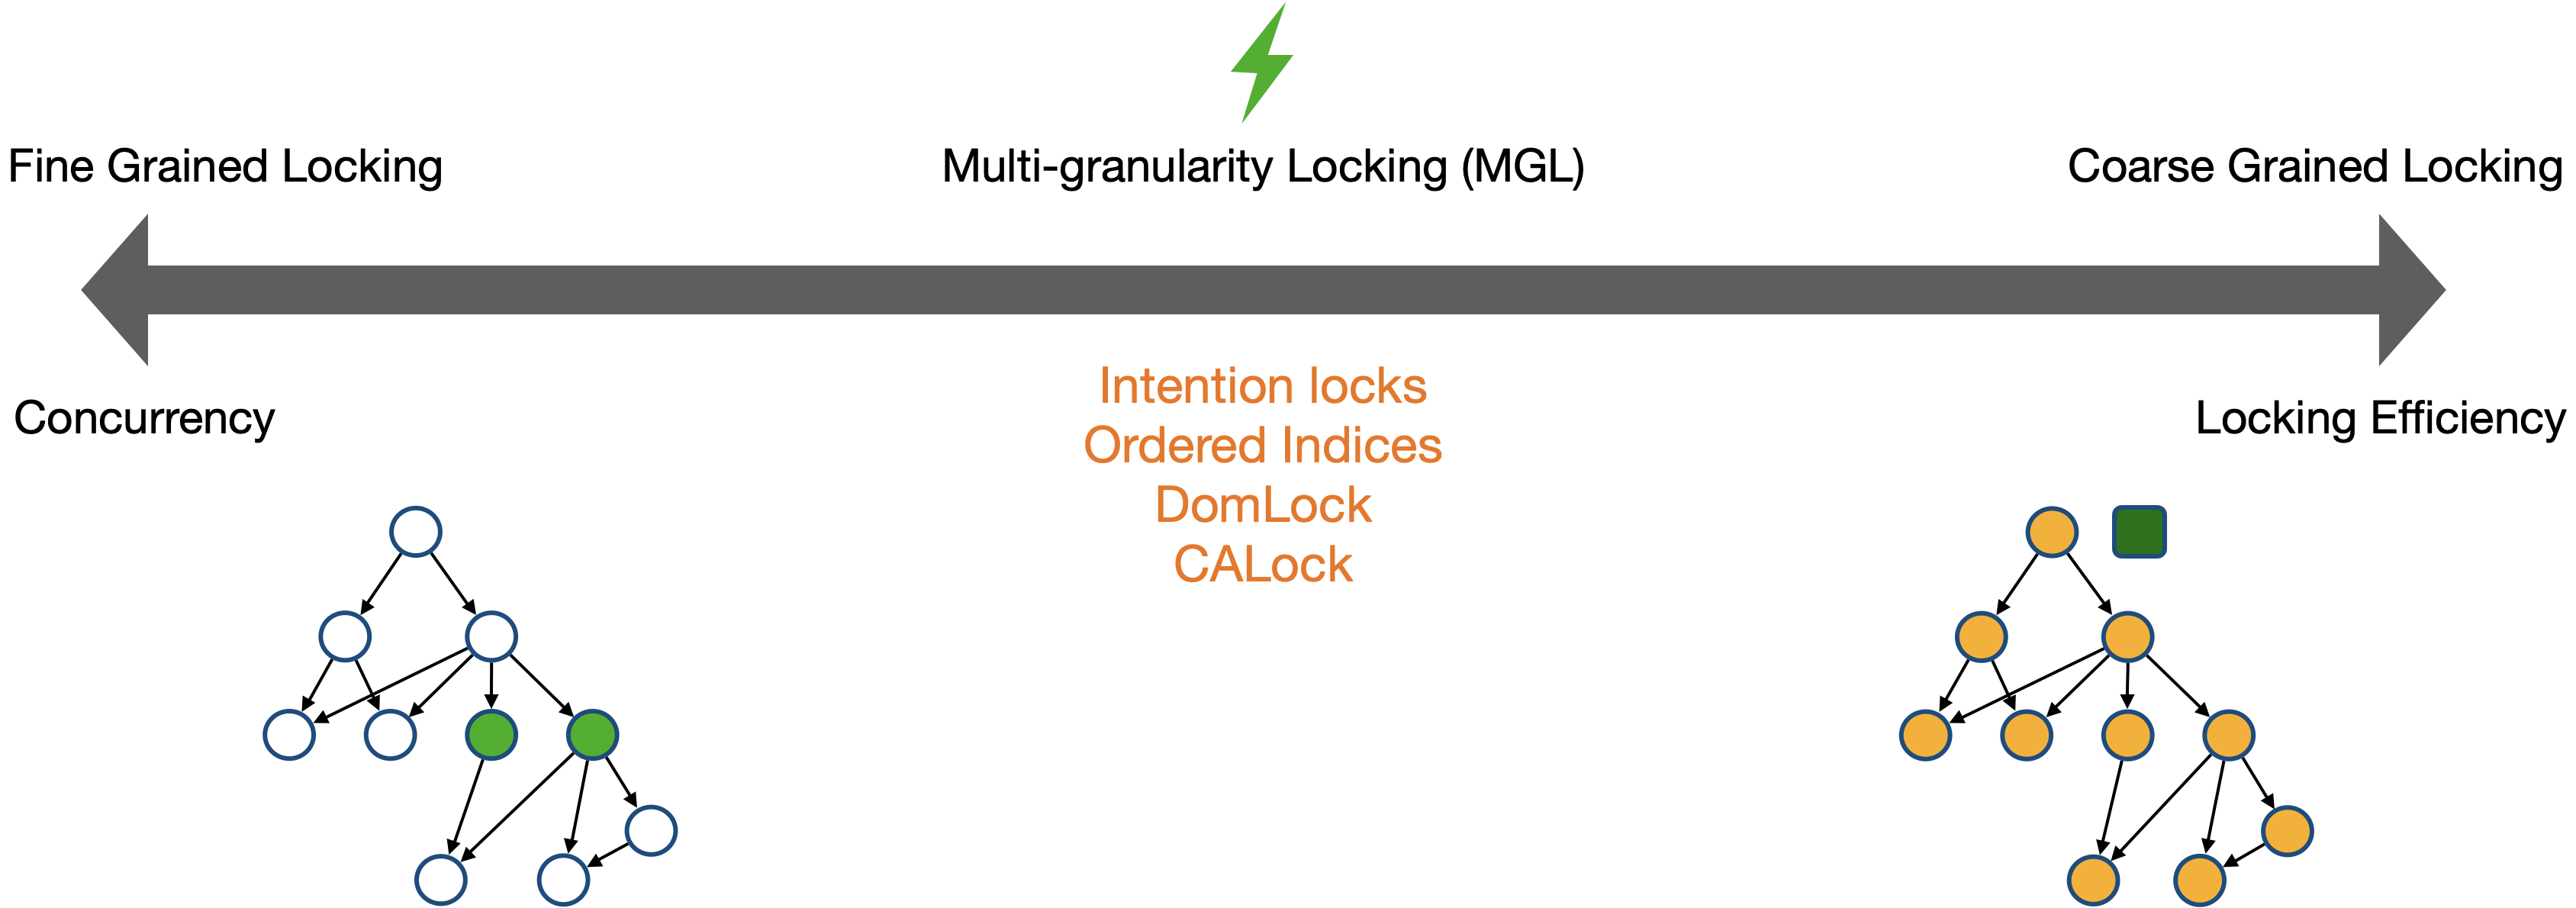
\includegraphics[width=\textwidth]{figures/MGLSpectrum.png}
    \label{fig:mglspectrum}
    \caption{Multi-Granularity locking provides a balance between Fine-grain and Coarse-grain locking.}
\end{figure}


% Another dimension of complexity with hierarchical data is the mutation of the hierarchy itself which causes topological changes.
% We refer to to such mutations as \emph{structural modifications}.
Structural modifications, which alter the topology of a hierarchy are especially challenging for MGL techniques. 
There already exist effective MGL protocols for hiaraarchies that do not undergo structural modifications, this is not the case for graphs whose structure can mutate. 
We discuss this in Chapter \ref{chap:relatedwork}.
% A structural modification operation adds or removes vertices and{\slash}or edges and may conflict with ordinary operations, or with another structural modification.
% Such operations affect the identification of lock granules as their size and shape now depend on the new topology of the graph.



% \section{Related Work}
% Survey of existing research on locking mechanisms and optimization techniques. Comparison of related approaches to the CALock algorithm.

